\documentclass{article}
\usepackage[paperwidth=188mm,paperheight=126mm,margin=4mm]{geometry}
\usepackage{graphicx}
\usepackage{tikz}
\usetikzlibrary{arrows.meta,positioning,fit,calc}
\pagestyle{empty}
\begin{document}
\noindent\resizebox{\textwidth}{!}{%
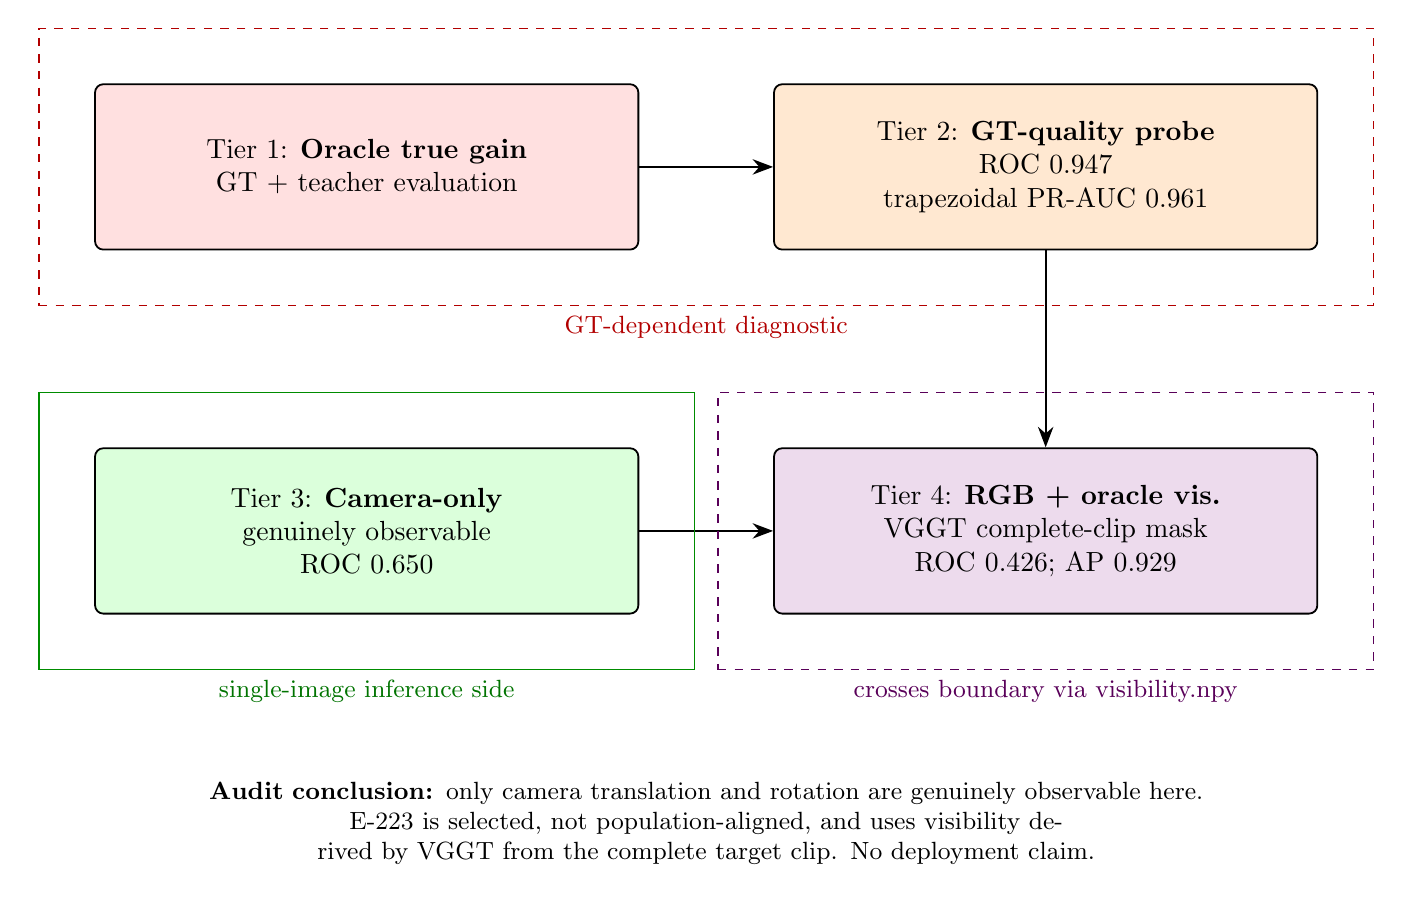
\begin{tikzpicture}[
  font=\normalsize,
  >={Stealth[length=2.6mm]},
  box/.style={rounded corners=3pt,draw,align=center,minimum height=21mm,minimum width=69mm,inner sep=5pt,line width=0.65pt},
  arr/.style={->,line width=0.8pt}
]
\node[box,fill=red!12] (oracle) {Tier 1: \textbf{Oracle true gain}\\GT + teacher evaluation};
\node[box,fill=orange!18,right=17mm of oracle] (probe) {Tier 2: \textbf{GT-quality probe}\\ROC 0.947\\trapezoidal PR-AUC 0.961};
\node[box,fill=green!14,below=25mm of oracle] (camera) {Tier 3: \textbf{Camera-only}\\genuinely observable\\ROC 0.650};
\node[box,fill=violet!14,right=17mm of camera] (rgbvis) {Tier 4: \textbf{RGB + oracle vis.}\\VGGT complete-clip mask\\ROC 0.426; AP 0.929};
\draw[arr] (oracle) -- (probe);
\draw[arr] (probe.south) to[out=-90,in=90] (rgbvis.north);
\draw[arr] (camera) -- (rgbvis);
\node[draw=red!70!black,dashed,fit=(oracle)(probe),inner sep=7mm,label={[font=\small,text=red!70!black]below:GT-dependent diagnostic}] {};
\node[draw=green!55!black,fit=(camera),inner sep=7mm,label={[font=\small,text=green!45!black]below:single-image inference side}] {};
\node[draw=violet!70!black,dashed,fit=(rgbvis),inner sep=7mm,label={[font=\small,text=violet!70!black]below:crosses boundary via visibility.npy}] {};
\node[font=\small,anchor=north,align=center,text width=170mm] at ($(camera.south)!0.5!(rgbvis.south)+(0,-20mm)$)
{\textbf{Audit conclusion:} only camera translation and rotation are genuinely observable here.\\E-223 is selected, not population-aligned, and uses visibility derived by VGGT from the complete target clip. No deployment claim.};
\end{tikzpicture}%
}
\end{document}
